\section{Python Exercise: DTFT Approximation using DFT}\label{sec:p6}


M=5000, 0.0005s vs 0.1s
M=5000, 0.0005s vs 2.7s


\begin{figure}[htbp]
	\centering
	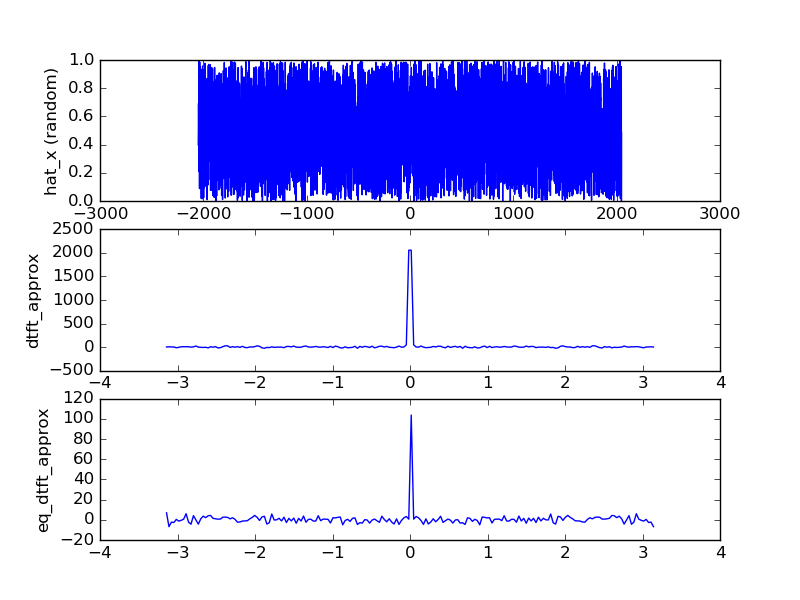
\includegraphics[width=\textwidth]{images/p6-1-200}
	\caption{}
	\label{fig:p6-1-200}
\end{figure}

\begin{figure}[htbp]
	\centering
	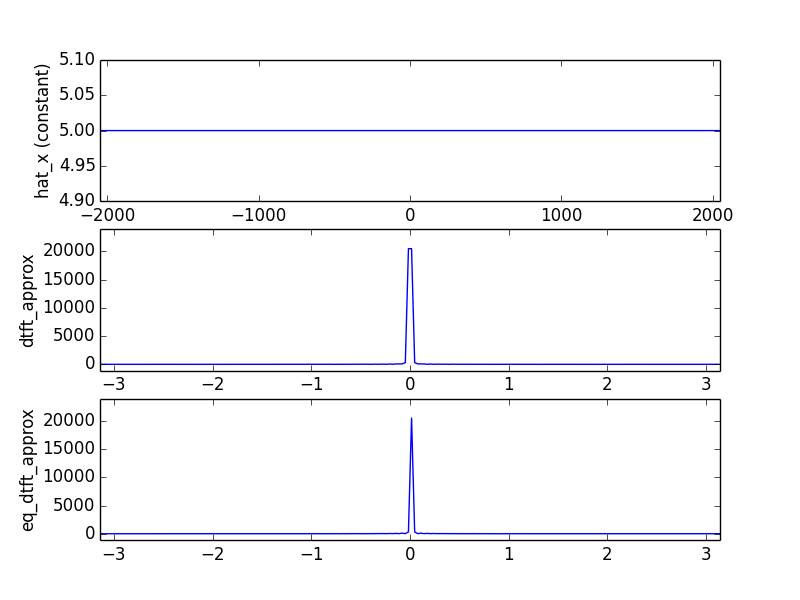
\includegraphics[width=\textwidth]{images/p6-2-200}
	\caption{}
	\label{fig:p6-2-200}
\end{figure}